% copied from the thesis chapter on fairness (content/fairness/fairness.tex, lines 504-766)
\begin{figure}[t]
\centering
\scalebox{0.72}{\begin{minipage}{\textwidth}%
\begin{subfigure}{0.4\textwidth}
\begin{center}
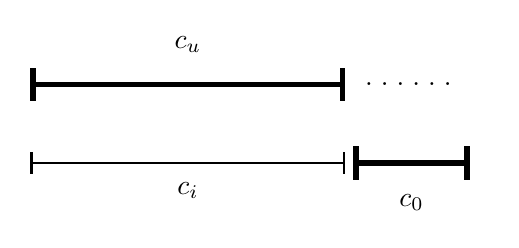
\begin{tikzpicture}
  \draw[line width=2, |-|]
  ({0.5}, 2.5) -- ({4.5}, 2.5) node[anchor=north west] {};
  \node at ({2.5}, 3) {$c_u$};
  \draw[line width=1, |-|]
  ({0.5}, 1.5) -- ({4.5}, 1.5) node[anchor=north west] {};
  \node at ({2.5},1.15) {$c_i$};
  \draw[line width=2, |-|]
  ({4.6}, 1.5) -- ({6.08}, 1.5) node[anchor=north west] {};
  \node at ({5.34}, 1.) {$c_0$};
  \node at ({5.3}, 3.) {};% {$c\in X$};
  \foreach \x in
    {
        1,2,3,4,5,6
    }
    {
        \node at ({4.6+\x*0.2}, 2.5) {$.$};
    }
\end{tikzpicture}
\caption{The vertex-selection day for $u\in V_i$, where $u \notin I$.
}
\end{center}
\end{subfigure}
\hspace{1cm}
\begin{subfigure}{0.4\textwidth}
\begin{center}
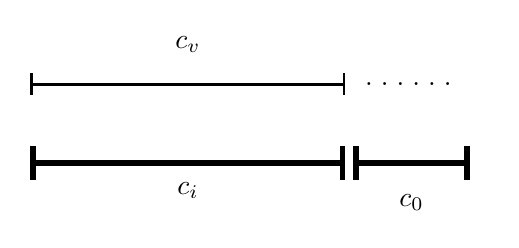
\begin{tikzpicture}
  \draw[line width=1, |-|]
  ({0.5}, 2.5) -- ({4.5}, 2.5) node[anchor=north west] {};
  \node at ({2.5}, 3) {$c_v$};
  \draw[line width=2, |-|]
  ({0.5}, 1.5) -- ({4.5}, 1.5) node[anchor=north west] {};
  \node at ({2.5},1.15) {$c_i$};
  \draw[line width=2, |-|]
  ({4.6}, 1.5) -- ({6.08}, 1.5) node[anchor=north west] {};
  \node at ({5.34}, 1.) {$c_0$};
  \node at ({5.3}, 3.) {};% {$c\in X$};
  \foreach \x in
    {
        1,2,3,4,5,6
    }
    {
        \node at ({4.6+\x*0.2}, 2.5) {$.$};
    }
\end{tikzpicture}
\caption{The vertex-selection day for $v\in V_i$, where $v \in I$.
}
\end{center}
\end{subfigure}

\vspace{0.5cm}

\begin{subfigure}{\textwidth}
\begin{center}
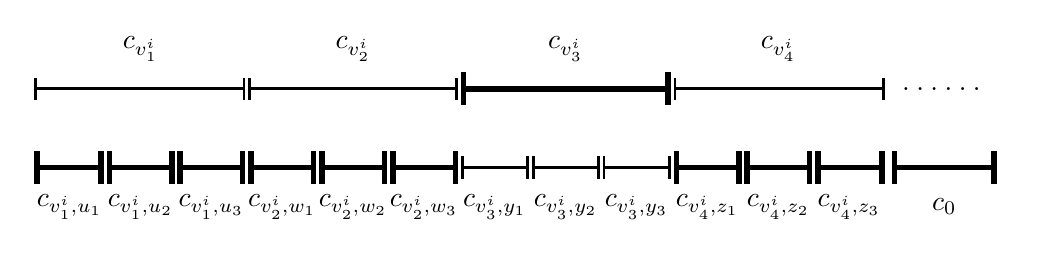
\begin{tikzpicture}[xscale=0.9]

  \draw[line width=1, |-|]
  ({0.5}, 2.5) -- ({3.48}, 2.5) node[anchor=north west] {};
  \node at ({2.}, 3) {$c_{v_1^i}$};
  \draw[line width=1, |-|]
  ({3.52}, 2.5) -- ({6.48}, 2.5) node[anchor=north west] {};
  \node at ({5.}, 3) {$c_{v_2^i}$};
  \draw[line width=2, |-|]
  ({6.52}, 2.5) -- ({9.48}, 2.5) node[anchor=north west] {};
  \node at ({8}, 3) {$c_{v_3^i}$};
  \draw[line width=1, |-|] ({9.52}, 2.5) -- ({12.5}, 2.5) node[anchor=north west] {};
  \node at ({11.}, 3) {$c_{v_4^i}$};

  \draw[line width=2, |-|]
  ({0.5}, 1.5) -- ({1.48}, 1.5) node[anchor=north west] {};
  \node at (1, 1.) {$c_{v_1^i,u_1}$};
  \draw[line width=2, |-|]
  ({1.52}, 1.5) -- ({2.48}, 1.5) node[anchor=north west] {};
  \node at (2, 1.) {$c_{v_1^i,u_2}$};
  \draw[line width=2, |-|]
  ({2.52}, 1.5) -- ({3.48}, 1.5) node[anchor=north west] {};
  \node at (3, 1.) {$c_{v_1^i,u_3}$};

  \draw[line width=2, |-|]
  ({3.52}, 1.5) -- ({4.48}, 1.5) node[anchor=north west] {};
  \node at (4, 1.) {$c_{v_2^i,w_1}$};
  \draw[line width=2, |-|]
  ({4.52}, 1.5) -- ({5.48}, 1.5) node[anchor=north west] {};
  \node at (5, 1.) {$c_{v_2^i,w_2}$};
  \draw[line width=2, |-|]
  ({5.52}, 1.5) -- ({6.48}, 1.5) node[anchor=north west] {};
  \node at (6, 1.) {$c_{v_2^i,w_3}$};

  \draw[line width=1, |-|]
  ({6.52}, 1.5) -- ({7.48}, 1.5) node[anchor=north west] {};
  \node at (7, 1.) {$c_{v_3^i,y_1}$};
  \draw[line width=1, |-|]
  ({7.52}, 1.5) -- ({8.48}, 1.5) node[anchor=north west] {};
  \node at (8, 1.) {$c_{v_3^i,y_2}$};
  \draw[line width=1, |-|]
  ({8.52}, 1.5) -- ({9.48}, 1.5) node[anchor=north west] {};
  \node at (9, 1.) {{$c_{v_3^i,y_3}$}};

  \draw[line width=2, |-|]
  ({9.52}, 1.5) -- ({10.48}, 1.5) node[anchor=north west] {};
  \node at (10, 1.) {{$c_{v_4^i,z_1}$}};
  \draw[line width=2, |-|]
  ({10.52}, 1.5) -- ({11.48}, 1.5) node[anchor=north west] {};
  \node at (11, 1.) {$c_{v_4^i,z_2}$};
  \draw[line width=2, |-|]
  ({11.52}, 1.5) -- ({12.5}, 1.5) node[anchor=north west] {};
  \node at (12, 1.) {$c_{v_4^i,z_3}$};

  \draw[line width=2, |-|]
  ({12.6}, 1.5) -- ({14.08}, 1.5) node[anchor=north west] {};
  \node at ({13.34}, 1.) {$c_0$};
  \node at ({13.3}, 3.) {};% {$c\in X$};
  \foreach \x in
    {
        1,2,3,4,5,6
    }
    {
        \node at ({12.6+\x*0.2}, 2.5) {$.$};
    }
\end{tikzpicture}
\caption{The $i$-th validation day where $v^i_3\in I$.}
\end{center}
\end{subfigure}

    

    
  
  
  
  

\end{minipage}}
\caption{An example of schedules on the vertex selection days and the validation days given a multicoloured independent set $I$. We mark in \textbf{bold} the jobs which are scheduled; the jobs not appearing in the gadget are shown schematically by dots, are pairwise disjoint and are all contained in the job of client $c_0$. }
\label{fig:vsg}%
\end{figure}
